\chapter{Porifera, Cnidaria,
Ctenophora}\label{porifera-cnidaria-ctenophora}

\section{Animals}\label{animals}

\href{https://en.wikipedia.org/wiki/Animal}{Animals} are eukaryotic,
multicellular organisms that form the biological kingdom Animalia. With
few exceptions, animals are motile (able to move), heterotrophic
(consume organic material), reproduce sexually, and their embryonic
development includes a blastula stage. The body plan of the animal
derives from this blastula, differentiating specialized tissues and
organs as it develops; this plan eventually becomes fixed, although some
undergo metamorphosis at some stage in their lives.

Zoology is the study of animals. Currently there are over 66,000
(less than 5\% of all animals) vertebrate species, and over 1.3 million
(over 95\% of all animals) invertebrate species in existence.
Classification of animals into groups (taxonomy) is accomplished using
either the hierarchical Linnaean system; or cladistics, which displays
diagrams (phylogenetic trees) called cladograms to show relationships
based on the evolutionary principle of the most recent common ancestor.
Some recent classifications based on modern cladistics have explicitly
abandoned the term ``kingdom'', noting that the traditional kingdoms are
not monophyletic, i.e., do not consist of all the descendants of a
common ancestor.

Animals are divided by body plan into vertebrates and invertebrates.
Vertebrates---fishes, amphibians, reptiles, birds, and mammals---have a
vertebral column (spine); invertebrates do not. All vertebrates and most
invertebrates are bilaterally symmetrical (Bilateria). Invertebrates
include arthropods, molluscs, roundworms, ringed worms, flatworms, and
other phyla in Ecdysozoa and Spiralia. Echinoderm larvae are initially
bilaterally symmetrical, but later as adults develop radial symmetry;
Cnidarians are radially symmetrical; ctenophores are biradially
symmetrical; and sponges have no symmetry.

Animal phyla appeared in the fossil record as marine species during the
Cambrian explosion, about 542 million years ago. Animals emerged as a
clade within \href{https://en.wikipedia.org/wiki/Apoikozoa}{Apoikozoa} as the sister group to the choanoflagellates.

\section{Poriphera}\label{poriphera}

\href{https://en.wikipedia.org/wiki/Sponge}{Sponges}, the members of the
phylum Porifera (meaning ``pore bearer''), are multicellular organisms
that have bodies full of pores and channels allowing water to circulate
through them, consisting of jelly-like mesohyl sandwiched between two
thin layers of cells. Sponges have unspecialized cells that can
transform into other types and that often migrate between the main cell
layers and the mesohyl in the process. Sponges do not have nervous,
digestive or circulatory systems. Instead, most rely on maintaining a
constant water flow through their bodies to obtain food and oxygen and
to remove wastes. Sponges are thought to be the first to branch off the
evolutionary tree from the common ancestor of all animals, making them
the sister group of all other animals.

The phylum Porifera is further divided into four classes mainly
according to the composition of their skeletons:

\begin{enumerate}
\def\labelenumi{\arabic{enumi}.}
\tightlist
\item
  Hexactinellida (glass sponges) have silicate spicules, the largest of
  which have six rays and may be individual or fused. The main
  components of their bodies are syncytia in which large numbers of cell
  share a single external membrane.
\item
  Calcarea have skeletons made of calcite, a form of calcium carbonate,
  which may form separate spicules or large masses. All the cells have a
  single nucleus and membrane.
\item
  Most Demospongiae have silicate spicules or spongin fibers or both
  within their soft tissues. However a few also have massive external
  skeletons made of aragonite, another form of calcium carbonate. All
  the cells have a single nucleus and membrane.
\item
  Archeocyatha are known only as fossils from the Cambrian period.
\end{enumerate}

Sponges are similar to other animals in that they are multicellular,
heterotrophic, lack cell walls and produce sperm cells. Unlike other
animals, they lack true tissues and organs, and have no body symmetry.
The shapes of their bodies are adapted for maximal efficiency of water
flow through the central cavity, where it deposits nutrients, and leaves
through a hole called the osculum. Many sponges have internal skeletons
of spongin and/or spicules of calcium carbonate or silicon dioxide. All
sponges are sessile aquatic animals. Although there are freshwater
species, the great majority are marine (salt water) species, ranging
from tidal zones to depths exceeding 8,800 m (5.5 mi).

While most of the approximately 5,000--10,000 known species feed on
bacteria and other food particles in the water, some host
photosynthesizing micro-organisms as endosymbionts and these alliances
often produce more food and oxygen than they consume. A few species of
sponge that live in food-poor environments have become carnivores that
prey mainly on small crustaceans.

\begin{figure}

{\centering 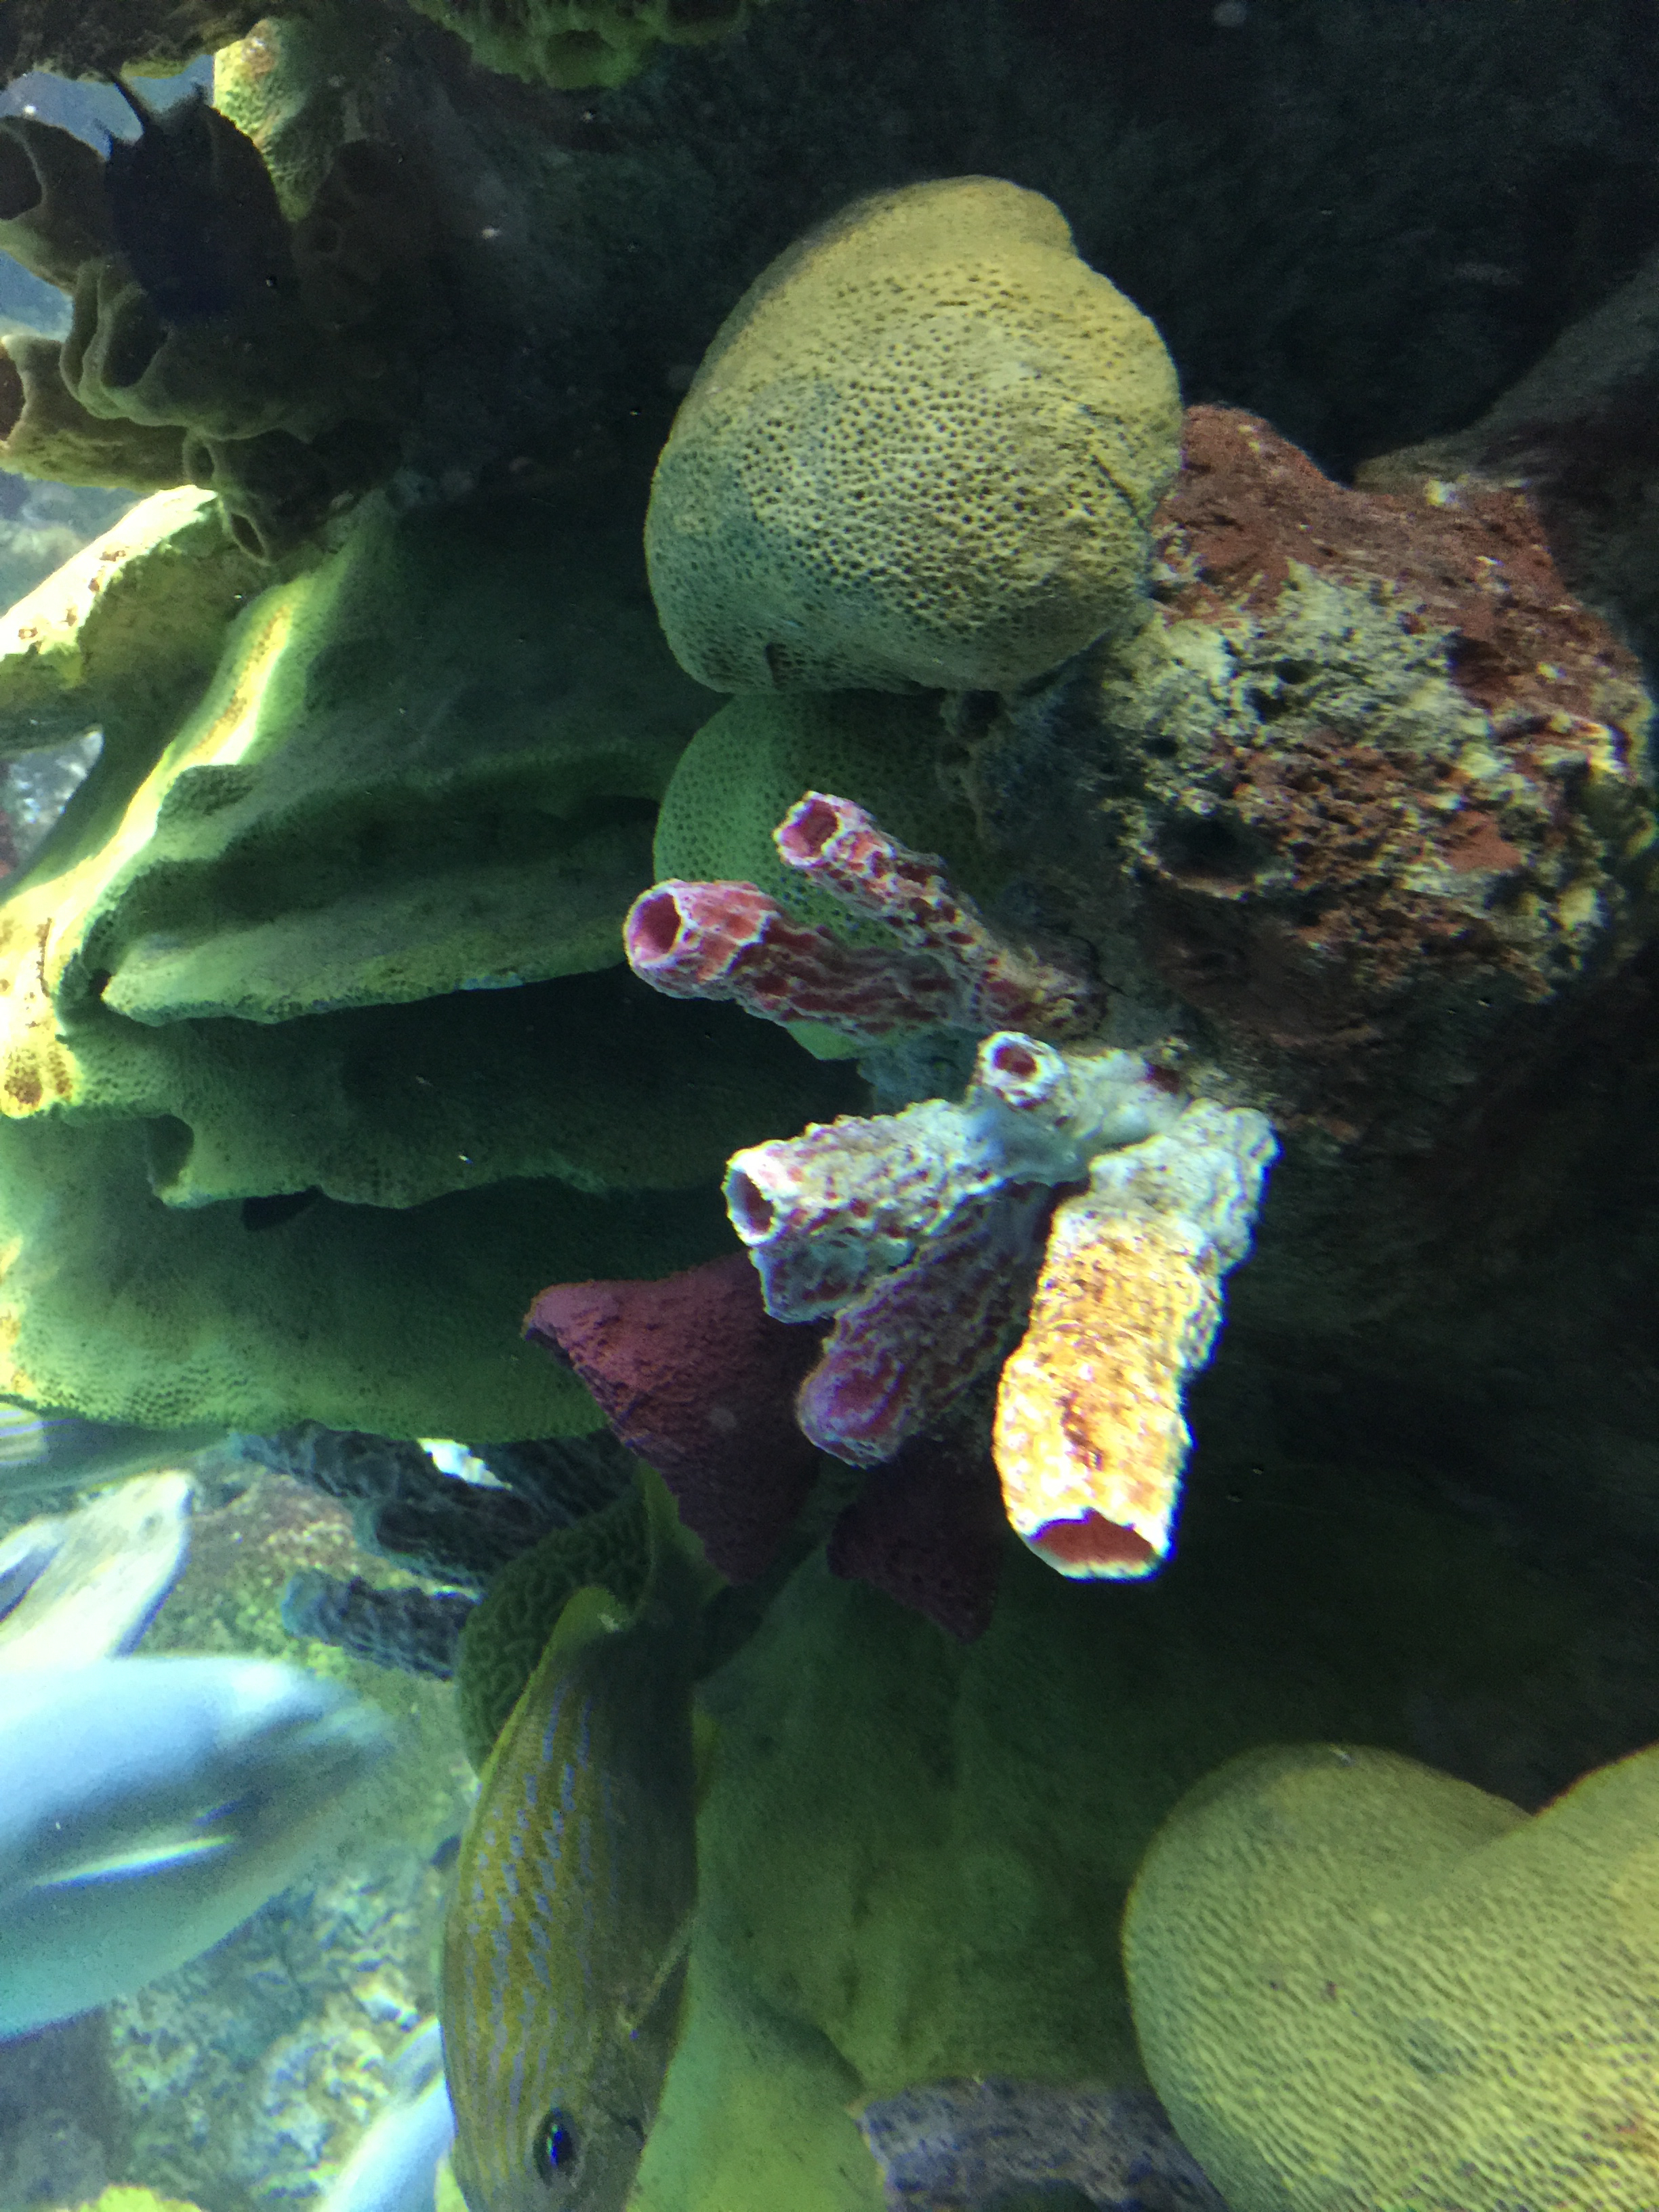
\includegraphics[width=0.7\linewidth]{./figures/porifera/sponges}

}

\caption{Sponges and corals.}\label{fig:sponges}
\end{figure}

Sponges in temperate regions live for at most a few years, but some
tropical species and perhaps some deep-ocean ones may live for 200 years
or more. Some calcified demosponges grow by only 0.2 mm (0.0079 in) per
year and, if that rate is constant, specimens 1 m (3.3 ft) wide must be
about 5,000 years old. Some sponges start sexual reproduction when only
a few weeks old, while others wait until they are several years old.

Most species use sexual reproduction, releasing sperm cells into the
water to fertilize ova that in some species are released and in others
are retained by the ``mother''. The fertilized eggs form larvae which
swim off in search of places to settle. Sponges are known for
regenerating from fragments that are broken off, although this only
works if the fragments include the right types of cells. A few species
reproduce by budding. When conditions deteriorate, for example as
temperatures drop, many freshwater species and a few marine ones produce
gemmules, ``survival pods'' of unspecialized cells that remain dormant
until conditions improve and then either form completely new sponges or
recolonize the skeletons of their parents.

The mesohyl functions as an endoskeleton in most sponges, and is the
only skeleton in soft sponges that encrust hard surfaces such as rocks.
More commonly, the mesohyl is stiffened by mineral spicules, by spongin
fibers or both. Demosponges use spongin, and in many species, silica
spicules and in some species, calcium carbonate exoskeletons.
Demosponges constitute about 90\% of all known sponge species, including
all freshwater ones, and have the widest range of habitats. Calcareous
sponges, which have calcium carbonate spicules and, in some species,
calcium carbonate exoskeletons, are restricted to relatively shallow
marine waters where production of calcium carbonate is easiest. The
fragile glass sponges, with ``scaffolding'' of silica spicules, are
restricted to polar regions and the ocean depths where predators are
rare. Fossils of all of these types have been found in rocks dated from
580 million years ago.

The few species of demosponge that have entirely soft fibrous skeletons
with no hard elements have been used by humans over thousands of years
for several purposes, including as padding and as cleaning tools. By the
1950s, though, these had been overfished so heavily that the industry
almost collapsed, and most sponge-like materials are now synthetic.
Sponges and their microscopic endosymbionts are now being researched as
possible sources of medicines for treating a wide range of diseases.
Dolphins have been observed using sponges as tools while foraging.

A sponge's body is hollow and is held in shape by the mesohyl, a
jelly-like substance made mainly of collagen and reinforced by a dense
network of fibers also made of collagen. The inner surface is covered
with choanocytes, cells with cylindrical or conical collars surrounding
one flagellum per choanocyte. The wave-like motion of the whip-like
flagella drives water through the sponge's body. All sponges have ostia,
channels leading to the interior through the mesohyl, and in most
sponges these are controlled by tube-like porocytes that form closable
inlet valves. Pinacocytes, plate-like cells, form a single-layered
external skin over all other parts of the mesohyl that are not covered
by choanocytes, and the pinacocytes also digest food particles that are
too large to enter the ostia, while those at the base of the animal are
responsible for anchoring it.

The single-celled choanoflagellates resemble the choanocyte cells of
sponges which are used to drive their water flow systems and capture
most of their food. This along with phylogenetic studies of ribosomal
molecules have been used as morphological evidence to suggest sponges
are the sister group to the rest of animals. Some studies have shown
that sponges do not form a monophyletic group, in other words do not
include all and only the descendants of a common ancestor. Recent
phylogenetic analyses suggest that comb jellies rather than sponges are
the sister group to the rest of animals.

Most sponges work rather like chimneys: they take in water at the bottom
and eject it from the osculum (``little mouth'') at the top. Since
ambient currents are faster at the top, the suction effect that they
produce by Bernoulli's principle does some of the work for free. Sponges
can control the water flow by various combinations of wholly or
partially closing the osculum and ostia (the intake pores) and varying
the beat of the flagella, and may shut it down if there is a lot of sand
or silt in the water.

Although the layers of pinacocytes and choanocytes resemble the
epithelia of more complex animals, they are not bound tightly by
cell-to-cell connections or a basal lamina (thin fibrous sheet
underneath). The flexibility of these layers and re-modeling of the
mesohyl by lophocytes allow the animals to adjust their shapes
throughout their lives to take maximum advantage of local water
currents.

\subsection{Reproduction}\label{reproduction-1}

Sponges have three asexual methods of reproduction: after fragmentation;
by budding; and by producing gemmules. Fragments of sponges may be
detached by currents or waves. They use the mobility of their
pinacocytes and choanocytes and reshaping of the mesohyl to re-attach
themselves to a suitable surface and then rebuild themselves as small
but functional sponges over the course of several days. The same
capabilities enable sponges that have been squeezed through a fine cloth
to regenerate. A sponge fragment can only regenerate if it contains both
collencytes to produce mesohyl and archeocytes to produce all the other
cell types. A very few species reproduce by budding. Gemmules are
``survival pods'' which a few marine sponges and many freshwater species
produce by the thousands when dying and which some, mainly freshwater
species, regularly produce in autumn. Spongocytes make gemmules by
wrapping shells of spongin, often reinforced with spicules, round
clusters of archeocytes that are full of nutrients.

Most sponges are hermaphrodites (function as both sexes simultaneously),
although sponges have no gonads (reproductive organs). Sperm are
produced by choanocytes or entire choanocyte chambers that sink into the
mesohyl and form spermatic cysts while eggs are formed by transformation
of archeocytes, or of choanocytes in some species. Each egg generally
acquires a yolk by consuming ``nurse cells''. During spawning, sperm
burst out of their cysts and are expelled via the osculum. If they
contact another sponge of the same species, the water flow carries them
to choanocytes that engulf them but, instead of digesting them,
metamorphose to an ameboid form and carry the sperm through the mesohyl
to eggs, which in most cases engulf the carrier and its cargo.

A few species release fertilized eggs into the water, but most retain
the eggs until they hatch. There are four types of larvae, but all are
balls of cells with an outer layer of cells whose flagellae or cilia
enable the larvae to move. After swimming for a few days the larvae sink
and crawl until they find a place to settle. Most of the cells transform
into archeocytes and then into the types appropriate for their locations
in a miniature adult sponge.

Glass sponge embryos start by dividing into separate cells, but once 32
cells have formed they rapidly transform into larvae that externally are
ovoid with a band of cilia round the middle that they use for movement,
but internally have the typical glass sponge structure of spicules with
a cobweb-like main syncytium draped around and between them and
choanosyncytia with multiple collar bodies in the center. The larvae
then leave their parents' bodies.

\section{\texorpdfstring{\emph{Grantia}}{Grantia}}\label{grantia}

\href{https://en.wikipedia.org/wiki/Grantia}{\emph{Grantia}} is a genus
of calcareous sponges belonging to the family Grantiidae. Grantias
contain spicules and spongin fibers.

\section{\texorpdfstring{View Prepared Slides of \emph{Grantia}}{View Prepared Slides of Grantia}}\label{view-prepared-slides}

\begin{enumerate}
\def\labelenumi{\arabic{enumi}.}
\tightlist
\item
  \emph{Grantia} c.s. l.s. (Figures \ref{fig:grantiaxs} and
  \ref{fig:grantials})

  \begin{itemize}
  \tightlist
  \item
    Identify spongocoel, radial canals, ostium, incurrent canals, collar
    cells (choanocytes).
  \end{itemize}
\item
  \emph{Grantia} thick x.s.

  \begin{itemize}
  \tightlist
  \item
    Identify spongocoel, incurrent canals, ostium, radial canals, collar
    cells (choanocytes).
  \end{itemize}
\item
  \emph{Grantia} spicules x.s. (Figure \ref{fig:spicules})

  \begin{itemize}
  \tightlist
  \item
    Notice shape.
  \end{itemize}
\end{enumerate}

\begin{figure}

{\centering \includegraphics[width=0.7\linewidth]{./figures/porifera/grantia_xs}

}

\caption{\emph{Grantia} cross section.}\label{fig:grantiaxs}
\end{figure}

\begin{figure}

{\centering \includegraphics[width=0.7\linewidth]{./figures/porifera/grantia_ls}

}

\caption{\emph{Grantia} longitudinal section.}\label{fig:grantials}
\end{figure}

\begin{figure}

{\centering \includegraphics[width=0.7\linewidth]{./figures/porifera/spicules}

}

\caption{Spicules.}\label{fig:spicules}
\end{figure}

\section{Cnidaria}\label{cnidaria}

\href{https://en.wikipedia.org/wiki/Cnidaria}{Cnidaria} is a phylum
containing over 10,000 species of animals found exclusively in aquatic
(freshwater and marine) environments: they are predominantly marine
species. Their distinguishing feature is the presence of cnidocytes,
specialized cells that they use mainly for capturing prey. Their bodies
consist of mesoglea, a non-living jelly-like substance, sandwiched
between two layers of epithelium that are mostly one cell thick. They
have two basic body forms: swimming medusae (singuar: medusa) and
sessile polyps, both of which are radially symmetrical with mouths
surrounded by tentacles that bear cnidocytes. Both forms have a single
orifice and body cavity that are used for digestion and respiration.
Many cnidarian species produce colonies that are single organisms
composed of medusa-like or polyp-like zooids, or both (hence they are
trimorphic). Cnidarians' activities are coordinated by a decentralized
nerve net and simple receptors. Several free-swimming species of Cubozoa
and Scyphozoa possess balance-sensing statocysts, and some have simple
eyes. Statocysts are sac-like structure sensory structures containing a
mineralized mass (statolith) and numerous innervated sensory hairs
(setae). The statolith's inertia causes it to push against the setae
when the animal accelerates. Deflection of setae by the statolith in
response to gravity activates neurons, providing feedback to the animal
on change in orientation and allowing balance to be maintained.

\begin{figure}

{\centering 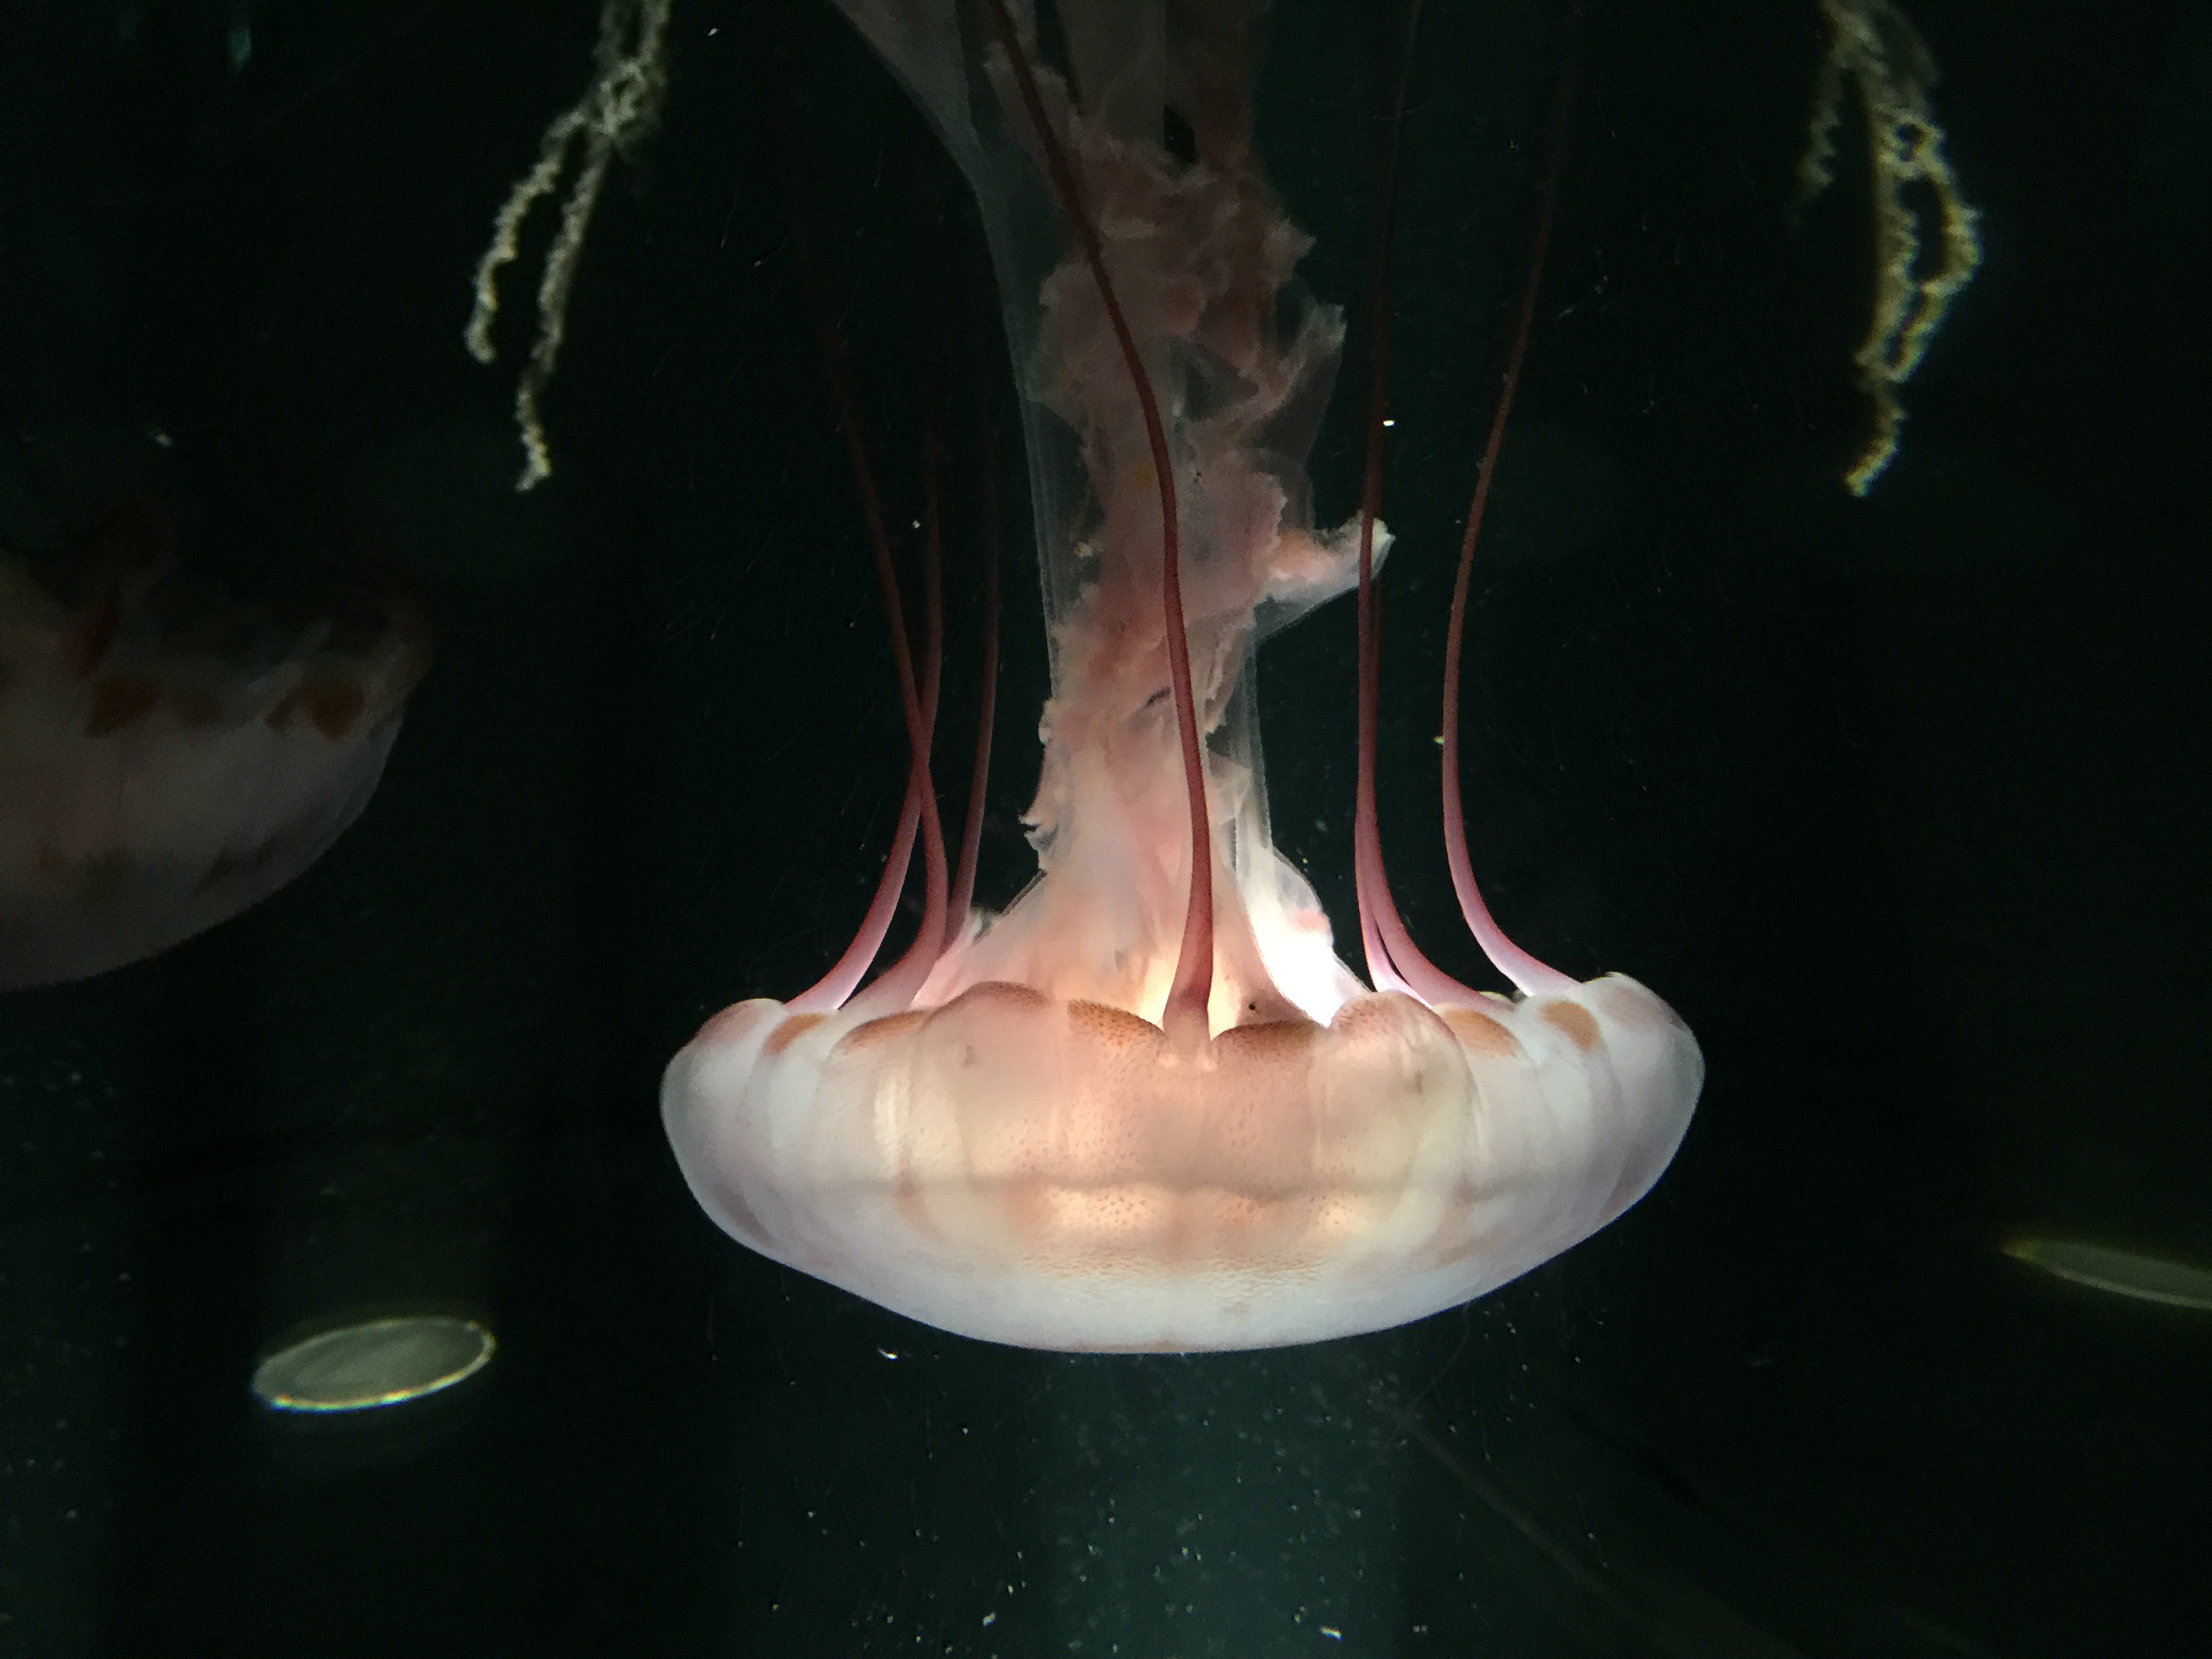
\includegraphics[width=0.7\linewidth]{./figures/porifera/chrysaora_colorata}

}

\caption{\href{https://en.wikipedia.org/wiki/Chrysaora_colorata}{Purple striped
jellyfish \emph{Chrysaora colorata}.}}\label{fig:chrysaora}
\end{figure}

Not all cnidarians reproduce sexually, with many species having complex
life cycles of asexual polyp stages and sexual medusae. Some, however,
omit either the polyp or the medusa stage.

Cnidarians are classified into five groups:

\begin{enumerate}
\def\labelenumi{\arabic{enumi}.}
\tightlist
\item
  Anthozoa (sea anemones, corals, sea pens)
\item
  Scyphozoa (jellyfish)
\item
  Cubozoa (box jellies)
\item
  Hydrozoa (a diverse group that includes all the freshwater
  cnidarians, such as \emph{Hydra}, as well as many marine forms, and
  has both sessile members and colonial swimmers, such as the Portuguese
  Man o' War)
\item
  Staurozoa (stalked jellyfish that do not have an alternation of
  polyp and medusa life cycle phases but are instead interpreted as an
  attached medusa stage, with a life style more resembling that of
  polypoid forms)
\end{enumerate}

Most cnidarians prey on organisms ranging in size from plankton to
animals several times larger than themselves, but many obtain much of
their nutrition from dinoflagellates, and a few are parasites. Many are
preyed on by other animals including starfish, sea slugs, fish, turtles,
and even other cnidarians. Many scleractinian corals---which form the
structural foundation for coral reefs---possess polyps that are filled
with symbiotic photo-synthetic zooxanthellae. While reef-forming corals
are almost entirely restricted to warm and shallow marine waters, other
cnidarians can be found at great depths, in polar regions, and in
freshwater.

\begin{figure}

{\centering 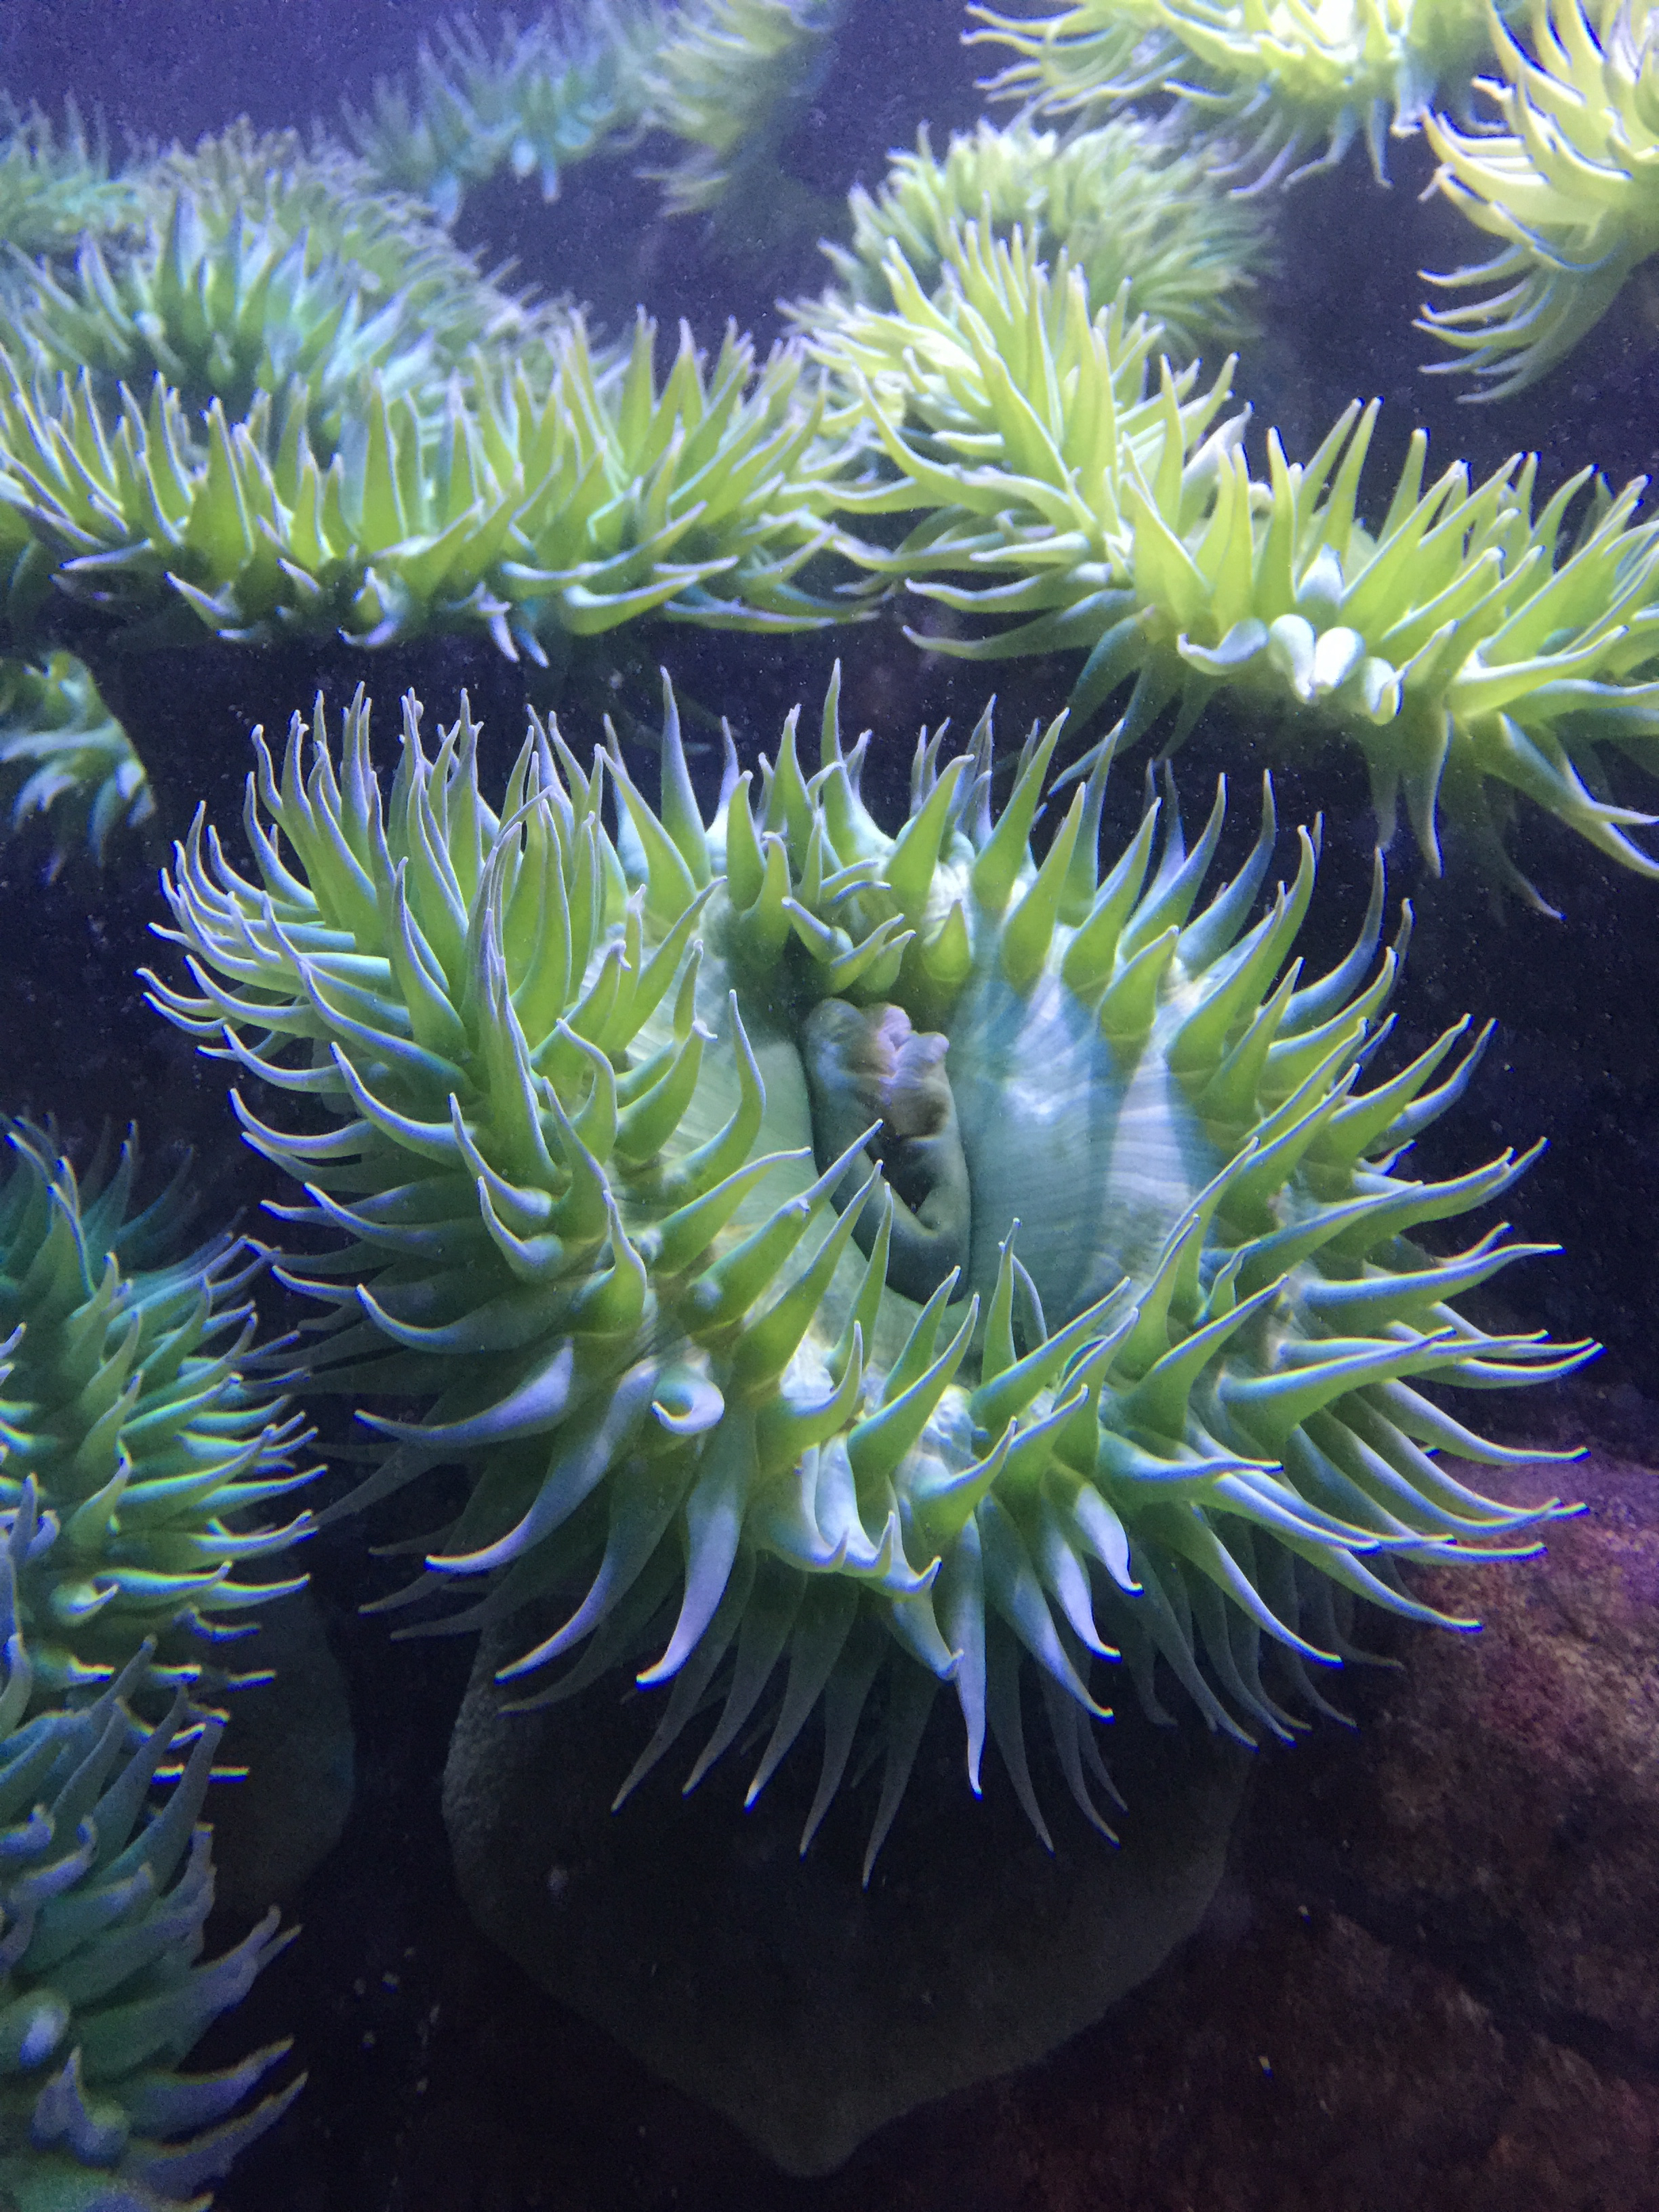
\includegraphics[width=0.7\linewidth]{./figures/porifera/anthopleura_xanthogrammica}

}

\caption{\href{https://en.wikipedia.org/wiki/Anthopleura_xanthogrammica}{Giant
green giant green anemone \emph{Anthopleura xanthogrammica}.}}\label{fig:anthopleura}
\end{figure}

Recent phylogenetic analyses support monophyly of cnidarians, as well as
the position of cnidarians as the sister group of bilaterians. Fossil
cnidarians have been found in rocks formed about 580 million years ago,
and other fossils show that corals may have been present shortly before
490 million years ago and diversified a few million years later.
However, molecular clock analysis of mitochondrial genes suggests a much
older age for the crown group of cnidarians, estimated around 741
million years ago, almost 200 million years before the Cambrian period
as well as any fossils.

\begin{figure}

{\centering \includegraphics[width=0.7\linewidth]{./figures/porifera/nematocyst}

}

\caption{\href{https://commons.wikimedia.org/wiki/File:Hydra_nematocyst_firing_01.png}{A
firing \emph{Hydra} nematocyst.}}\label{fig:nematocyst}
\end{figure}

\subsection{Reproduction}\label{reproduction-2}

Cnidarian sexual reproduction often involves a complex life cycle with
both polyp and medusa stages. For example, in Scyphozoa (jellyfish) and
Cubozoa (box jellies) larvae swim until they settle down and become
polyps. Polyps grow normally but then absorb their tentacles and split
horizontally into a series of disks that become juvenile medusae, a
process called strobilation. The juveniles swim off and slowly grow to
maturity, while the polyps re-grow and may continue strobilating
periodically. The adults have gonads in the gastroderm, and these
release ova and sperm into the water in the breeding season.

This phenomenon of succession of differently organized generations (one
asexually reproducing, sessile polyp, followed by a free-swimming medusa
or a sessile polyp that reproduces sexually) is sometimes called
``alternation of asexual and sexual phases'' or ``metagenesis'', but
should not be confused with the alternation of generations as found in
plants.

Shortened forms of this life cycle are common, for example some oceanic
scyphozoans omit the polyp stage completely, and cubozoan polyps produce
only one medusa. Hydrozoa have a variety of life cycles. Some have no
polyp stages and some (e.g.~\emph{Hydra}) have no medusae. In some species, the
medusae remain attached to the polyp and are responsible for sexual
reproduction; in extreme cases these reproductive zooids may not look
much like medusae. Meanwhile, life cycle reversal, in which polyps are
formed directly from medusae without the involvement of sexual
reproduction process, was observed in both Hydrozoa (Turritopsis dohrnii
and Laodicea undulata) and Scyphozoa (e. g. \emph{Aurelia}. Anthozoa have
no medusa stage at all and the polyps are responsible for sexual
reproduction.

Spawning is generally driven by environmental factors such as changes in
the water temperature, and their release is triggered by lighting
conditions such as sunrise, sunset or the phase of the moon. Many
species of Cnidaria may spawn simultaneously in the same location, so
that there are too many ova and sperm for predators to eat more than a
tiny percentage --- one famous example is the Great Barrier Reef, where
at least 110 corals and a few non-cnidarian invertebrates produce enough
gametes to turn the water cloudy. These mass spawnings may produce
hybrids, some of which can settle and form polyps, but it is not known
how long these can survive. In some species the ova release chemicals
that attract sperm of the same species.

The fertilized eggs develop into larvae by dividing until there are
enough cells to form a hollow sphere (blastula) and then a depression
forms at one end (gastrulation) and eventually becomes the digestive
cavity. However, in cnidarians the depression forms at the end further
from the yolk (at the animal pole), while in bilaterians it forms at the
other end (vegetal pole). The larvae, called planulae, swim or crawl by
means of cilia. They are cigar-shaped but slightly broader at the
``front'' end, which is the aboral, vegetal-pole end and eventually
attaches to a substrate if the species has a polyp stage.

Anthozoan larvae either have large yolks or are capable of feeding on
plankton, and some already have endosymbiotic algae that help to feed
them. Since the parents are immobile, these feeding capabilities extend
the larvae's range and avoid overcrowding of sites. Scyphozoan and
hydrozoan larvae have little yolk and most lack endosymbiotic algae, and
therefore have to settle quickly and metamorphose into polyps. Instead,
these species rely on their medusae to extend their ranges.

All known cnidaria can reproduce asexually by various means, in addition
to regenerating after being fragmented. Hydrozoan polyps only bud, while
the medusae of some hydrozoans can divide down the middle. Scyphozoan
polyps can both bud and split down the middle. In addition to both of
these methods, Anthozoa can split horizontally just above the base.
Asexual reproduction makes the daughter cnidarian a clone of the adult.

\section{\texorpdfstring{\emph{Hydra}}{Hydra}}\label{hydra}

\href{https://en.wikipedia.org/wiki/Hydra_(genus)}{\emph{Hydra}} is a
genus of small, fresh-water organisms of the phylum Cnidaria and class
Hydrozoa. They are native to the temperate and tropical regions.
Biologists are especially interested in \emph{Hydra} because of their
regenerative ability --- they do not appear to die of old age, or indeed
to age at all. Hydra has a tubular, radially symmetric body up to 10 mm
long when extended, secured by a simple adhesive foot called the basal
disc. Gland cells in the basal disc secrete a sticky fluid that accounts
for its adhesive properties.

At the free end of the body is a mouth opening surrounded by one to
twelve thin, mobile tentacles. Each tentacle, or cnida (plural: cnidae),
is clothed with highly specialized stinging cells called cnidocytes.
Cnidocytes contain specialized structures called nematocysts, which look
like miniature light bulbs with a coiled thread inside. At the narrow
outer edge of the cnidocyte is a short trigger hair called a cnidocil.
Upon contact with prey, the contents of the nematocyst are explosively
discharged, firing a dart-like thread containing neurotoxins into
whatever triggered the release which can paralyse the prey, especially
if many hundreds of nematocysts are fired.

\emph{Hydra} has two main body layers, which makes it ``diploblastic''.
The layers are separated by mesoglea, a gel-like substance. The outer
layer is the epidermis, and the inner layer is called the gastrodermis,
because it lines the stomach. The cells making up these two body layers
are relatively simple. Hydramacin is a bactericide recently discovered
in \emph{Hydra}; it protects the outer layer against infection.

The nervous system of \emph{\emph{Hydra}} is a nerve net, which is structurally
simple compared to more derived animal nervous systems. \emph{Hydra}
does not have a recognizable brain or true muscles. Nerve nets connect
sensory photoreceptors and touch-sensitive nerve cells located in the
body wall and tentacles.

Respiration and excretion occur by diffusion everywhere through the
epidermis.

If \emph{Hydra} are alarmed or attacked, the tentacles can be retracted
to small buds, and the body column itself can be retracted to a small
gelatinous sphere. \emph{Hydra} generally react in the same way
regardless of the direction of the stimulus, and this may be due to the
simplicity of the nerve nets.

\emph{Hydra} are generally sedentary or sessile, but do occasionally
move quite readily, especially when hunting.

\subsection{Reproduction and life
cycle}\label{reproduction-and-life-cycle}

When food is plentiful, many \emph{Hydra} reproduce asexually by
producing buds in the body wall, which grow to be miniature adults and
break away when they are mature. When a hydra is well fed, a new bud can
form every two days. When conditions are harsh, often before winter or
in poor feeding conditions, sexual reproduction occurs in some
\emph{Hydra}. Swellings in the body wall develop into either an ovary or
testes. The testes release free-swimming gametes into the water, and
these can fertilize the egg in the ovary of another individual. The
fertilized eggs secrete a tough outer coating, and, as the adult dies
(due to starvation and/or cold), these resting eggs fall to the bottom
of the lake or pond to await better conditions, whereupon they hatch
into nymph \emph{Hydra}. Some, like \emph{Hydra circumcincta} and
\emph{Hydra viridissima}, are hermaphrodites and may produce both testes
and an ovary at the same time.

Many members of the Hydrozoa go through a body change from a polyp to an
adult form called a medusa. However, all \emph{Hydra}, despite being
hydrozoans, remain as polyps throughout their lives.

\begin{figure}

{\centering \includegraphics[width=0.7\linewidth]{./figures/porifera/hydra}

}

\caption{\href{https://en.wikipedia.org/wiki/Hydra_(genus)\#/media/File:Hydra-Foto.jpg}{A
budding \emph{Hydra}.}}\label{fig:hydra}
\end{figure}

\section{\texorpdfstring{View Prepared Slides of
\emph{Hydra}}{View Prepared Slides of Hydra}}\label{view-prepared-slides-of-hydra}

\begin{enumerate}
\def\labelenumi{\arabic{enumi}.}
\tightlist
\item
  \emph{Hydra} x.s. (Figure \ref{fig:hydraxs})

  \begin{itemize}
  \tightlist
  \item
    Identify: epidermis (ectoderm), gastrodermis (endoderm),
    gastrovascular cavity.
  \end{itemize}
\item
  \emph{Hydra} spermary (Figure \ref{fig:spermary})

  \begin{itemize}
  \tightlist
  \item
    Identify: testis, sperms, epidermis, mesoglea, gastrodermis,
    gastrovascular cavity.
  \end{itemize}
\end{enumerate}

\begin{figure}

{\centering \includegraphics[width=0.7\linewidth]{./figures/porifera/hydra_xs}

}

\caption{\emph{Hydra} cross section.}\label{fig:hydraxs}
\end{figure}

\begin{figure}

{\centering \includegraphics[width=0.7\linewidth]{./figures/porifera/hydra_spermary}

}

\caption{\emph{Aurelia} spermary}\label{fig:spermary}
\end{figure}

\section{\texorpdfstring{\emph{Aurelia}}{Aurelia}}\label{aurelia}

\href{https://en.wikipedia.org/wiki/Aurelia_(name)}{\emph{Aurelia}} is a genus
of scyphozoan jellyfish, commonly called moon jellies. Species of
Aurelia can be found in the Atlantic Ocean, the Arctic Ocean and the
Pacific Ocean, and are common to the waters off California, northern
China, Japan, Korea, Australia, New Zealand, the Black Sea, Indonesia,
the East Coast of the United States as well as Europe. Aurelia undergoes
alternation of generations, whereby the sexually-reproducing pelagic
medusa stage is either male or female, and the benthic polyp stage
reproduces asexually.

\section{\texorpdfstring{View Prepared Slides of
\emph{Aurelia}}{View Prepared Slides of Aurelia}}\label{view-prepared-slides-of-Aurelia}
\begin{enumerate}
\def\labelenumi{\arabic{enumi}.}
\tightlist
\item
  \emph{Aurelia} Planula (Figure \ref{fig:planula})
\item
  \emph{Aurelia} Scyphistoma (Figure \ref{fig:scyphistoma})

  \begin{itemize}
  \tightlist
  \item
    Identify: tentacles, and base.
  \end{itemize}
\item
  \emph{Aurelia} Strobilus (Figure \ref{fig:strobilus})

  \begin{itemize}
  \tightlist
  \item
    Identify: tentacles, base, developing medusae (ephyrae).
  \end{itemize}
\end{enumerate}

\begin{figure}

{\centering \includegraphics[width=0.7\linewidth]{./figures/porifera/aurelia_planula}

}

\caption{\emph{Aurelia} planula larva}\label{fig:planula}
\end{figure}

\begin{figure}

{\centering \includegraphics[width=0.7\linewidth]{./figures/porifera/aurelia_scyphistoma}

}

\caption{\emph{Aurelia} scyphistoma}\label{fig:scyphistoma}
\end{figure}

\begin{figure}

{\centering \includegraphics[width=0.7\linewidth]{./figures/porifera/aurelia_strobilus}

}

\caption{\emph{Aurelia} strobilus}\label{fig:strobilus}
\end{figure}

\section{\texorpdfstring{\emph{Obelia}}{Obelia}}\label{obelia}

\href{https://en.wikipedia.org/wiki/Obelia}{\emph{Obelia}} is a genus in the
class Hydrozoa, which consists of mainly marine and some freshwater
animal species and have both the polyp and medusa stages in their life
cycle. The genus belongs to the phylum Cnidaria, which are all aquatic
and mainly marine organisms that are relatively simple in structure. It
is also called sea fur. \emph{Obelia} has a worldwide distribution except the
high-arctic and Antarctic seas. The medusa stage of \emph{Obelia} species are
common in coastal and offshore plankton around the world. \emph{Obelia} are
usually found no deeper than 200 meters from the water's surface,
growing in intertidal rock pools and at the extreme low water of spring
tides.

Through its life cycle, \emph{Obelia} take two forms: polyp and medusa. They
are diploblastic, with two true tissue layers -- an epidermis
(ectodermis) and a gastrodermis (endodermis), with a jelly-like mesoglea
filling the area between the two true tissue layers. They carry a nerve
net with no brain or ganglia. A gastrovascular cavity is present where
the digestion starts and later becomes intracellular. They have
incomplete digestive tracts where the food enters, is digested, and
expelled through the same opening. During the polyp stage, the mouth is
situated at the top of the body, surrounded by tentacles, whereas during
the medusa stage, the mouth is situated at the distal end of the main
body structure. Four gonads lie in this main body structure, or
manubrium. When food is taken in through the mouth, it enters the
manubrium. The food is then distributed through a canal system,
consisting of four radial canals and an outer ring. Defense and the
capture of prey are helped by unique stinging cells called cnidocytes
that contain nematocysts, which are triggered by the cnidocil. It has a
ridge-like structure on the inner margin, called velum. If the velum is
present, it is named as craspedote medusa.

The polyp colony reproduces asexually. During this stage of life, \emph{Obelia}
are confined to substrate surfaces. On this mature colony there are
individual hydranths called gastrozooids, which can be found expanded or
contracted, to aid in the growth of this organism by feeding; the
reproductive polyp gonozooids has medusa buds. Other hydranths are
specialized for defense. The main stalky body of the colony is composed
of a coenosarc, which is covered by a protective perisarc.

The next generation of the life cycle begins when the medusae are
released from these gonozooids, producing free swimming only male
medusae velum with gonads, a mouth, and tentacles. The physical
appearance of the male and female medusae velum, including their gonads,
are indistinguishable, and the sex can only be determined by observing
the inside of the gonads, which will either contain sperm or eggs. The
medusae reproduce sexually, releasing sperm and eggs that fertilize to
form a zygote, which later morphs into a blastula, then a ciliated
swimming larva called a planula.

The planulae live free-swimming for a while but eventually attach
themselves to some solid surface, where they begin their reproductive
phase of life. Once attached to a substrate, a planula quickly develops
into one feeding polyp. As the polyp grows, it begins developing
branches of other feeding individuals, thus forming a new generation of
polyps by asexual budding.

\begin{figure}

{\centering 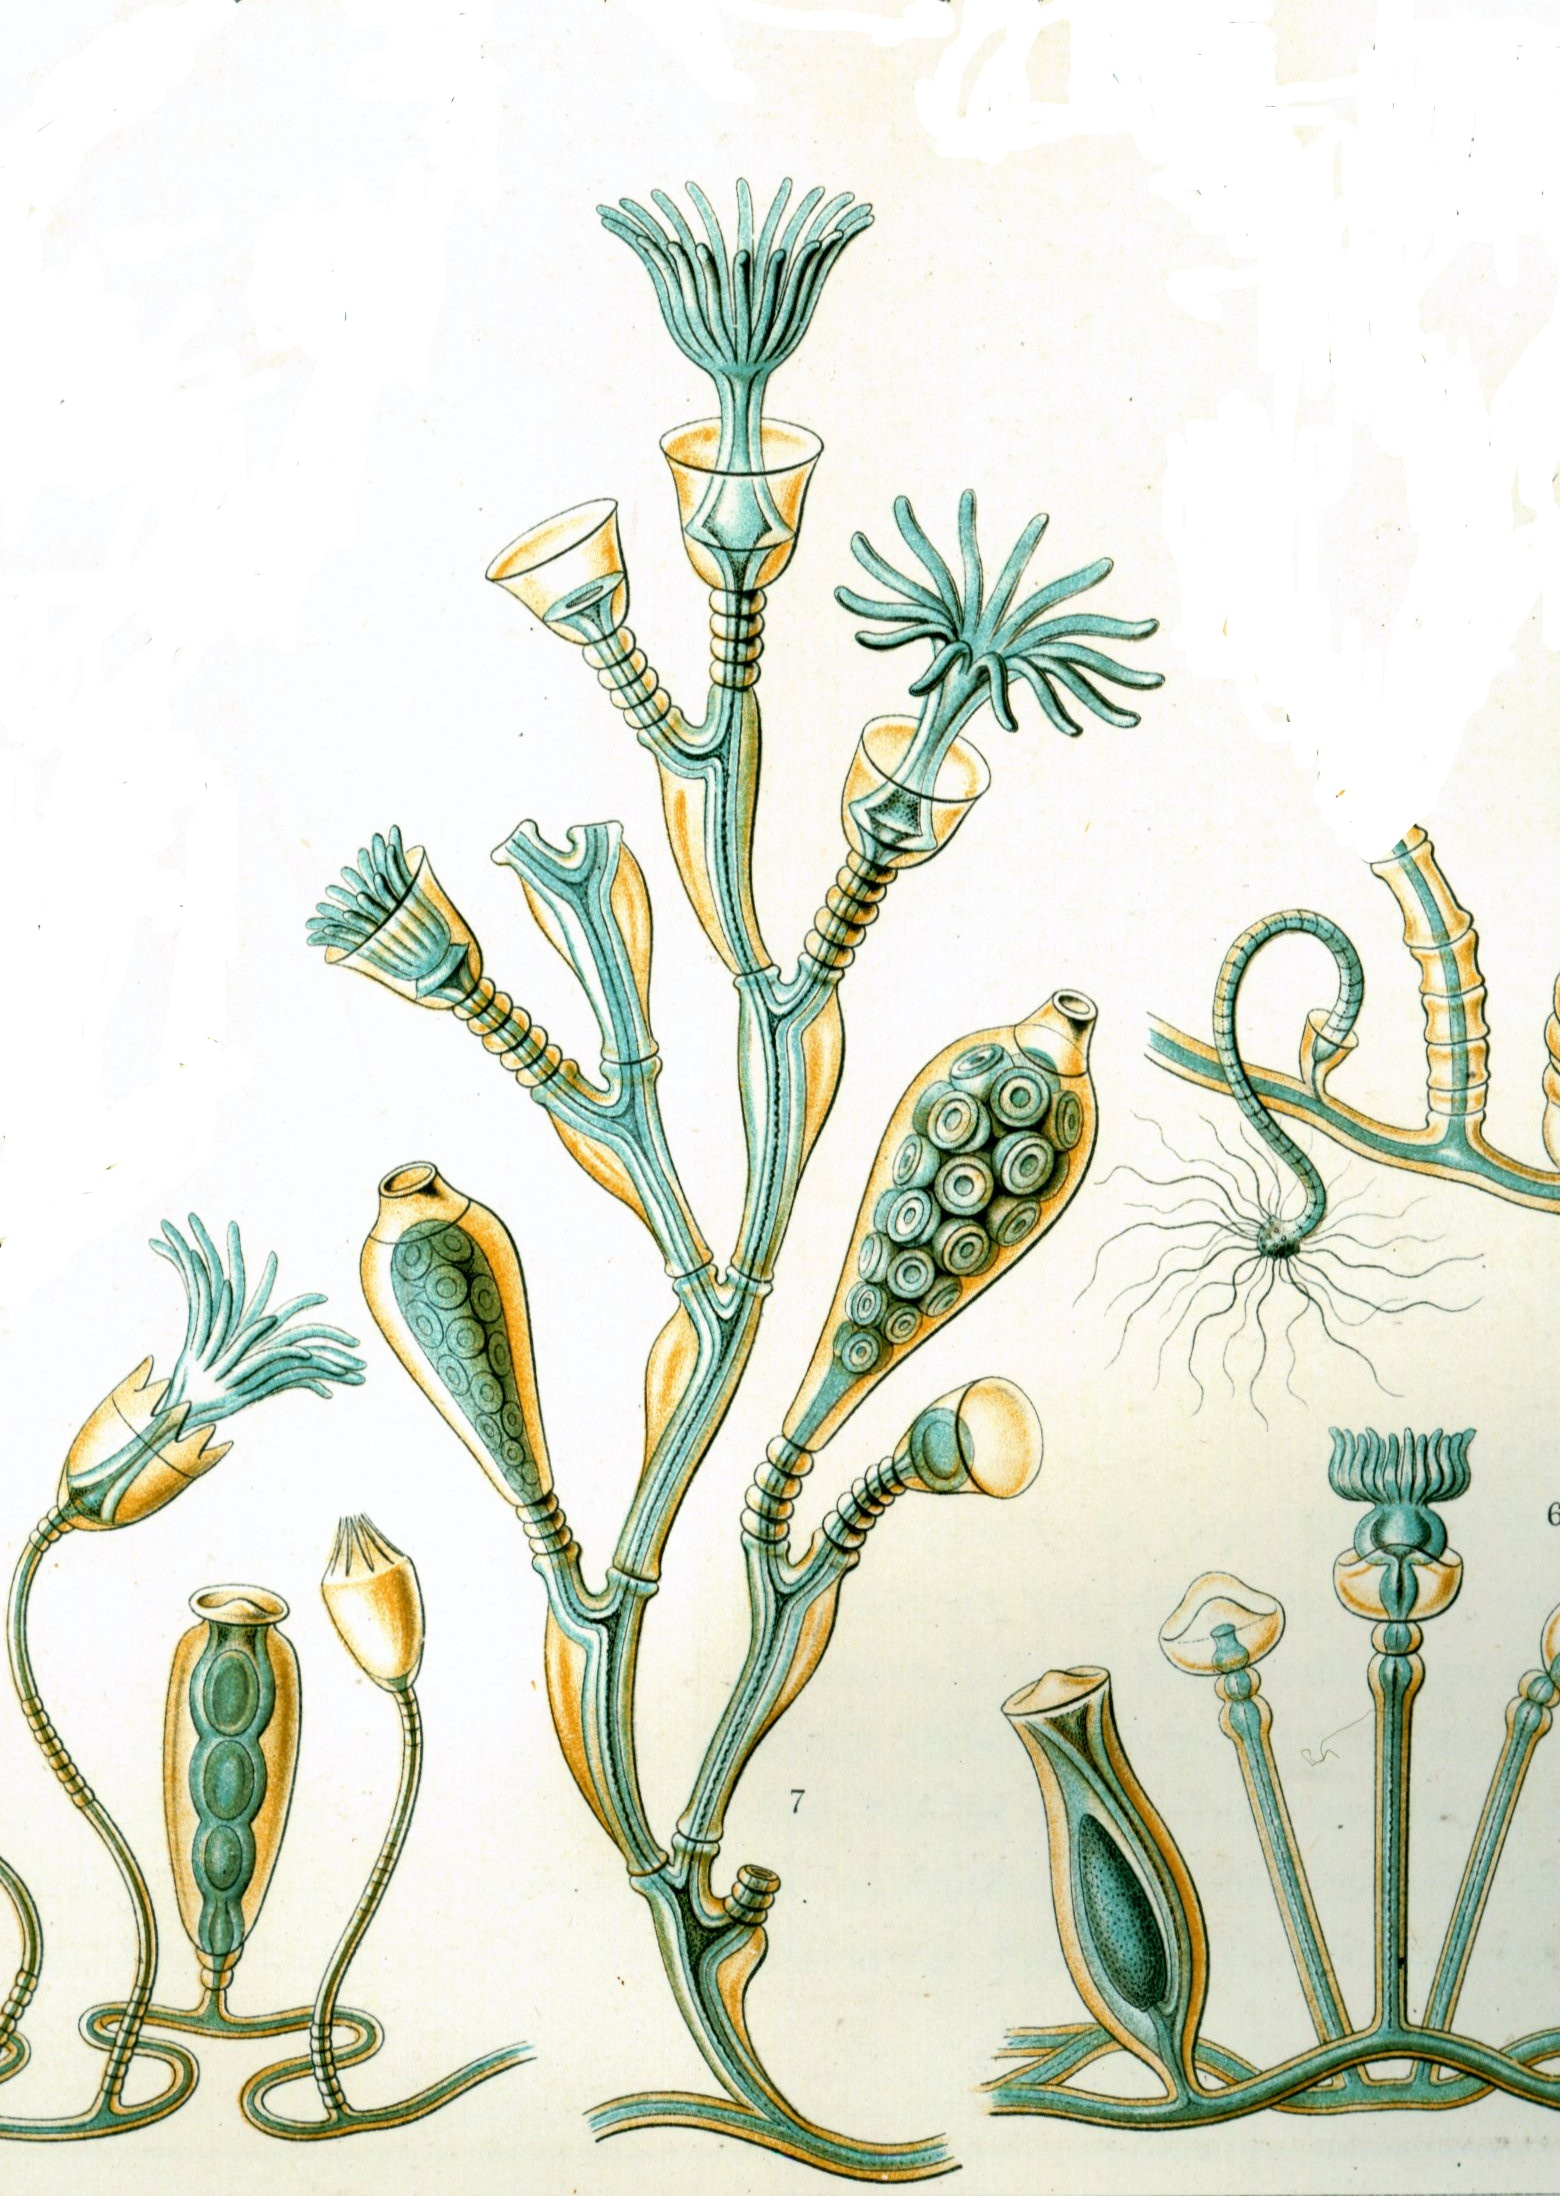
\includegraphics[width=0.7\linewidth]{./figures/porifera/obelia_geniculata}

}

\caption{\href{https://commons.wikimedia.org/wiki/File:Obelia_geniculata.jpg}{\emph{Obelia
geniculata} colony with 3 hydranths and 2 gonophores.}}\label{fig:obelia}
\end{figure}

\section{View Prepared Slides of
\emph{Obelia}}\label{view-prepared-slides-of-obelia}

\begin{enumerate}
\def\labelenumi{\arabic{enumi}.}
\tightlist
\item
  \emph{Obelia} medusa w.m. (Figure \ref{fig:obeliamedusa})

  \begin{itemize}
  \tightlist
  \item
    Identify: tentacles, manubrium, mouth, gonads.
  \end{itemize}
\item
  \emph{Obelia} w.m. (Figure \ref{fig:obeliacolony})

  \begin{itemize}
  \tightlist
  \item
    Identify: hydranth, tentacles, mouth, hydrotheca, gonangium,
    gonotheca, gonopore, medusa buds, blastostyle.
  \end{itemize}
\end{enumerate}



\begin{figure}

{\centering \includegraphics[width=0.7\linewidth]{./figures/porifera/obelia_medusa}

}

\caption{\emph{Obelia} medusa.}\label{fig:obeliamedusa}
\end{figure}



\begin{figure}

{\centering 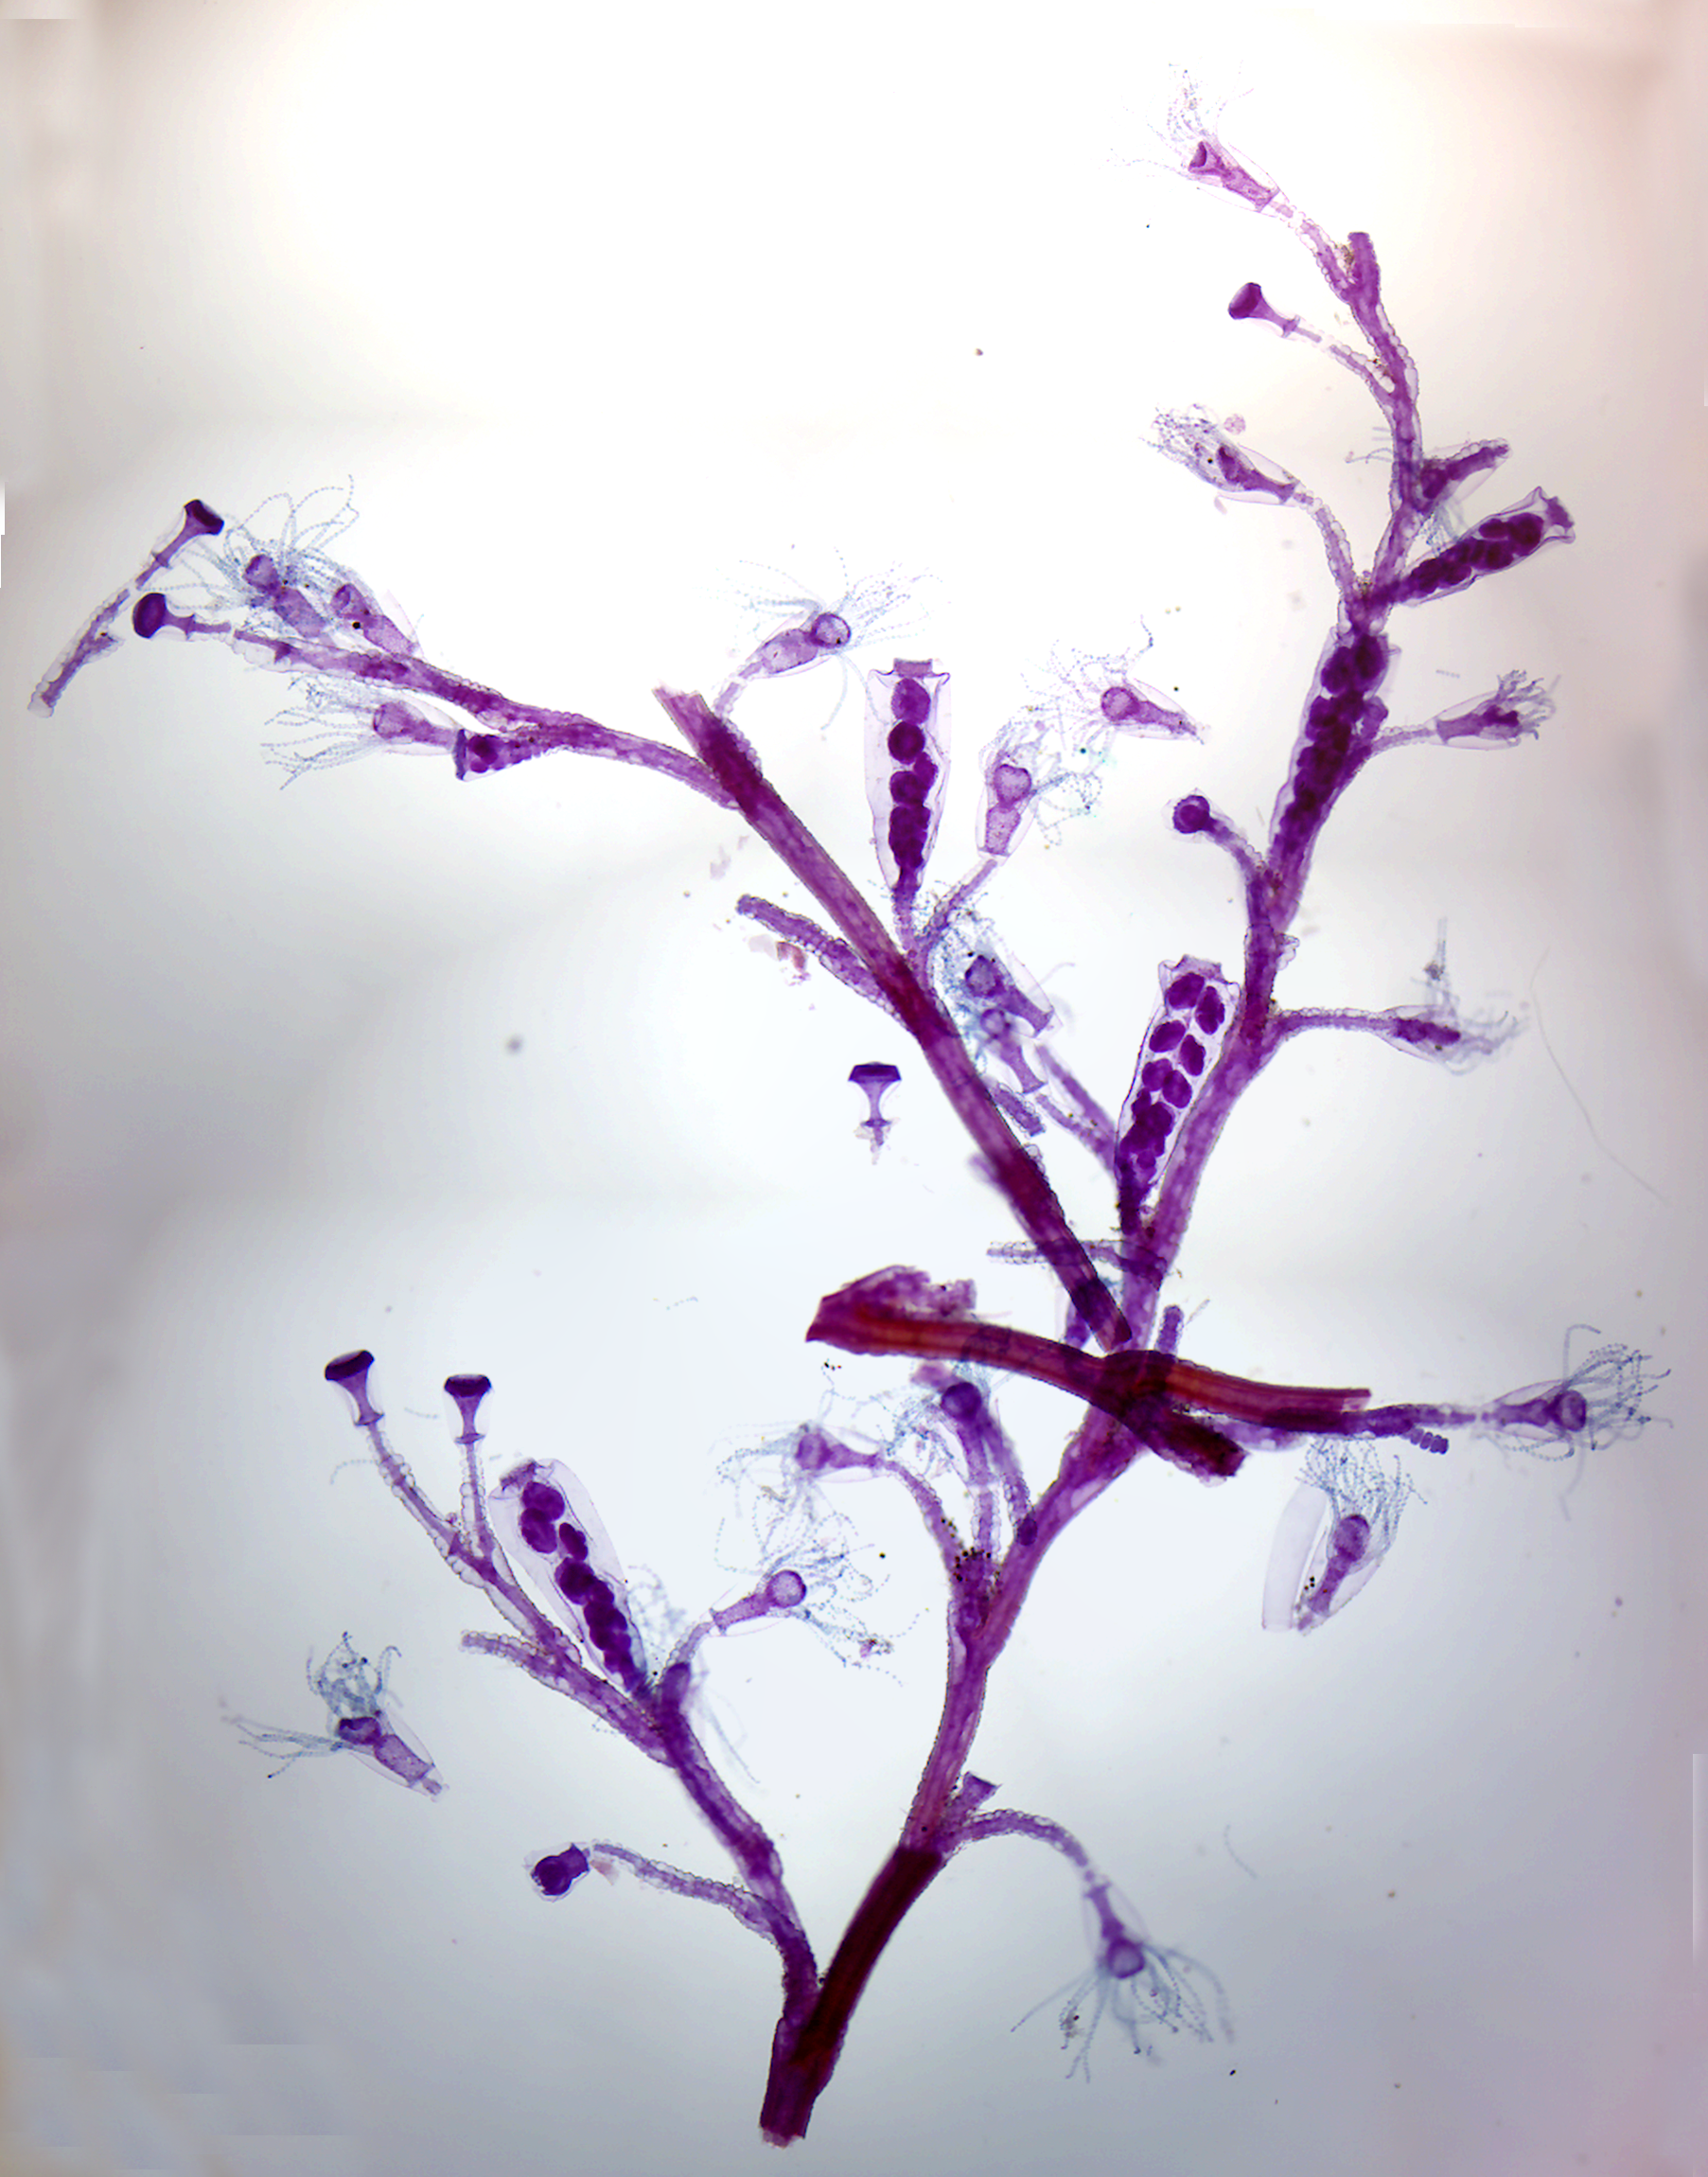
\includegraphics[width=0.7\linewidth]{./figures/porifera/obelia_wm}

}

\caption{\emph{Obelia} colony.}\label{fig:obeliacolony}
\end{figure}

\section{\texorpdfstring{\emph{Metridium}}{Metridium}}\label{metridium}

Members of the genus
\href{https://en.wikipedia.org/wiki/Metridium}{Metridium}, also known as
plumose anemones, are sea anemones found mostly in the cooler waters of
the northern Pacific and Atlantic oceans. They are characterized by
their numerous threadlike tentacles extending from atop a smooth
cylindrical column, and can vary from a few centimeters in height up to
one meter or more. In larger specimens, the oral disk becomes densely
curved and frilly.

\begin{figure}

{\centering 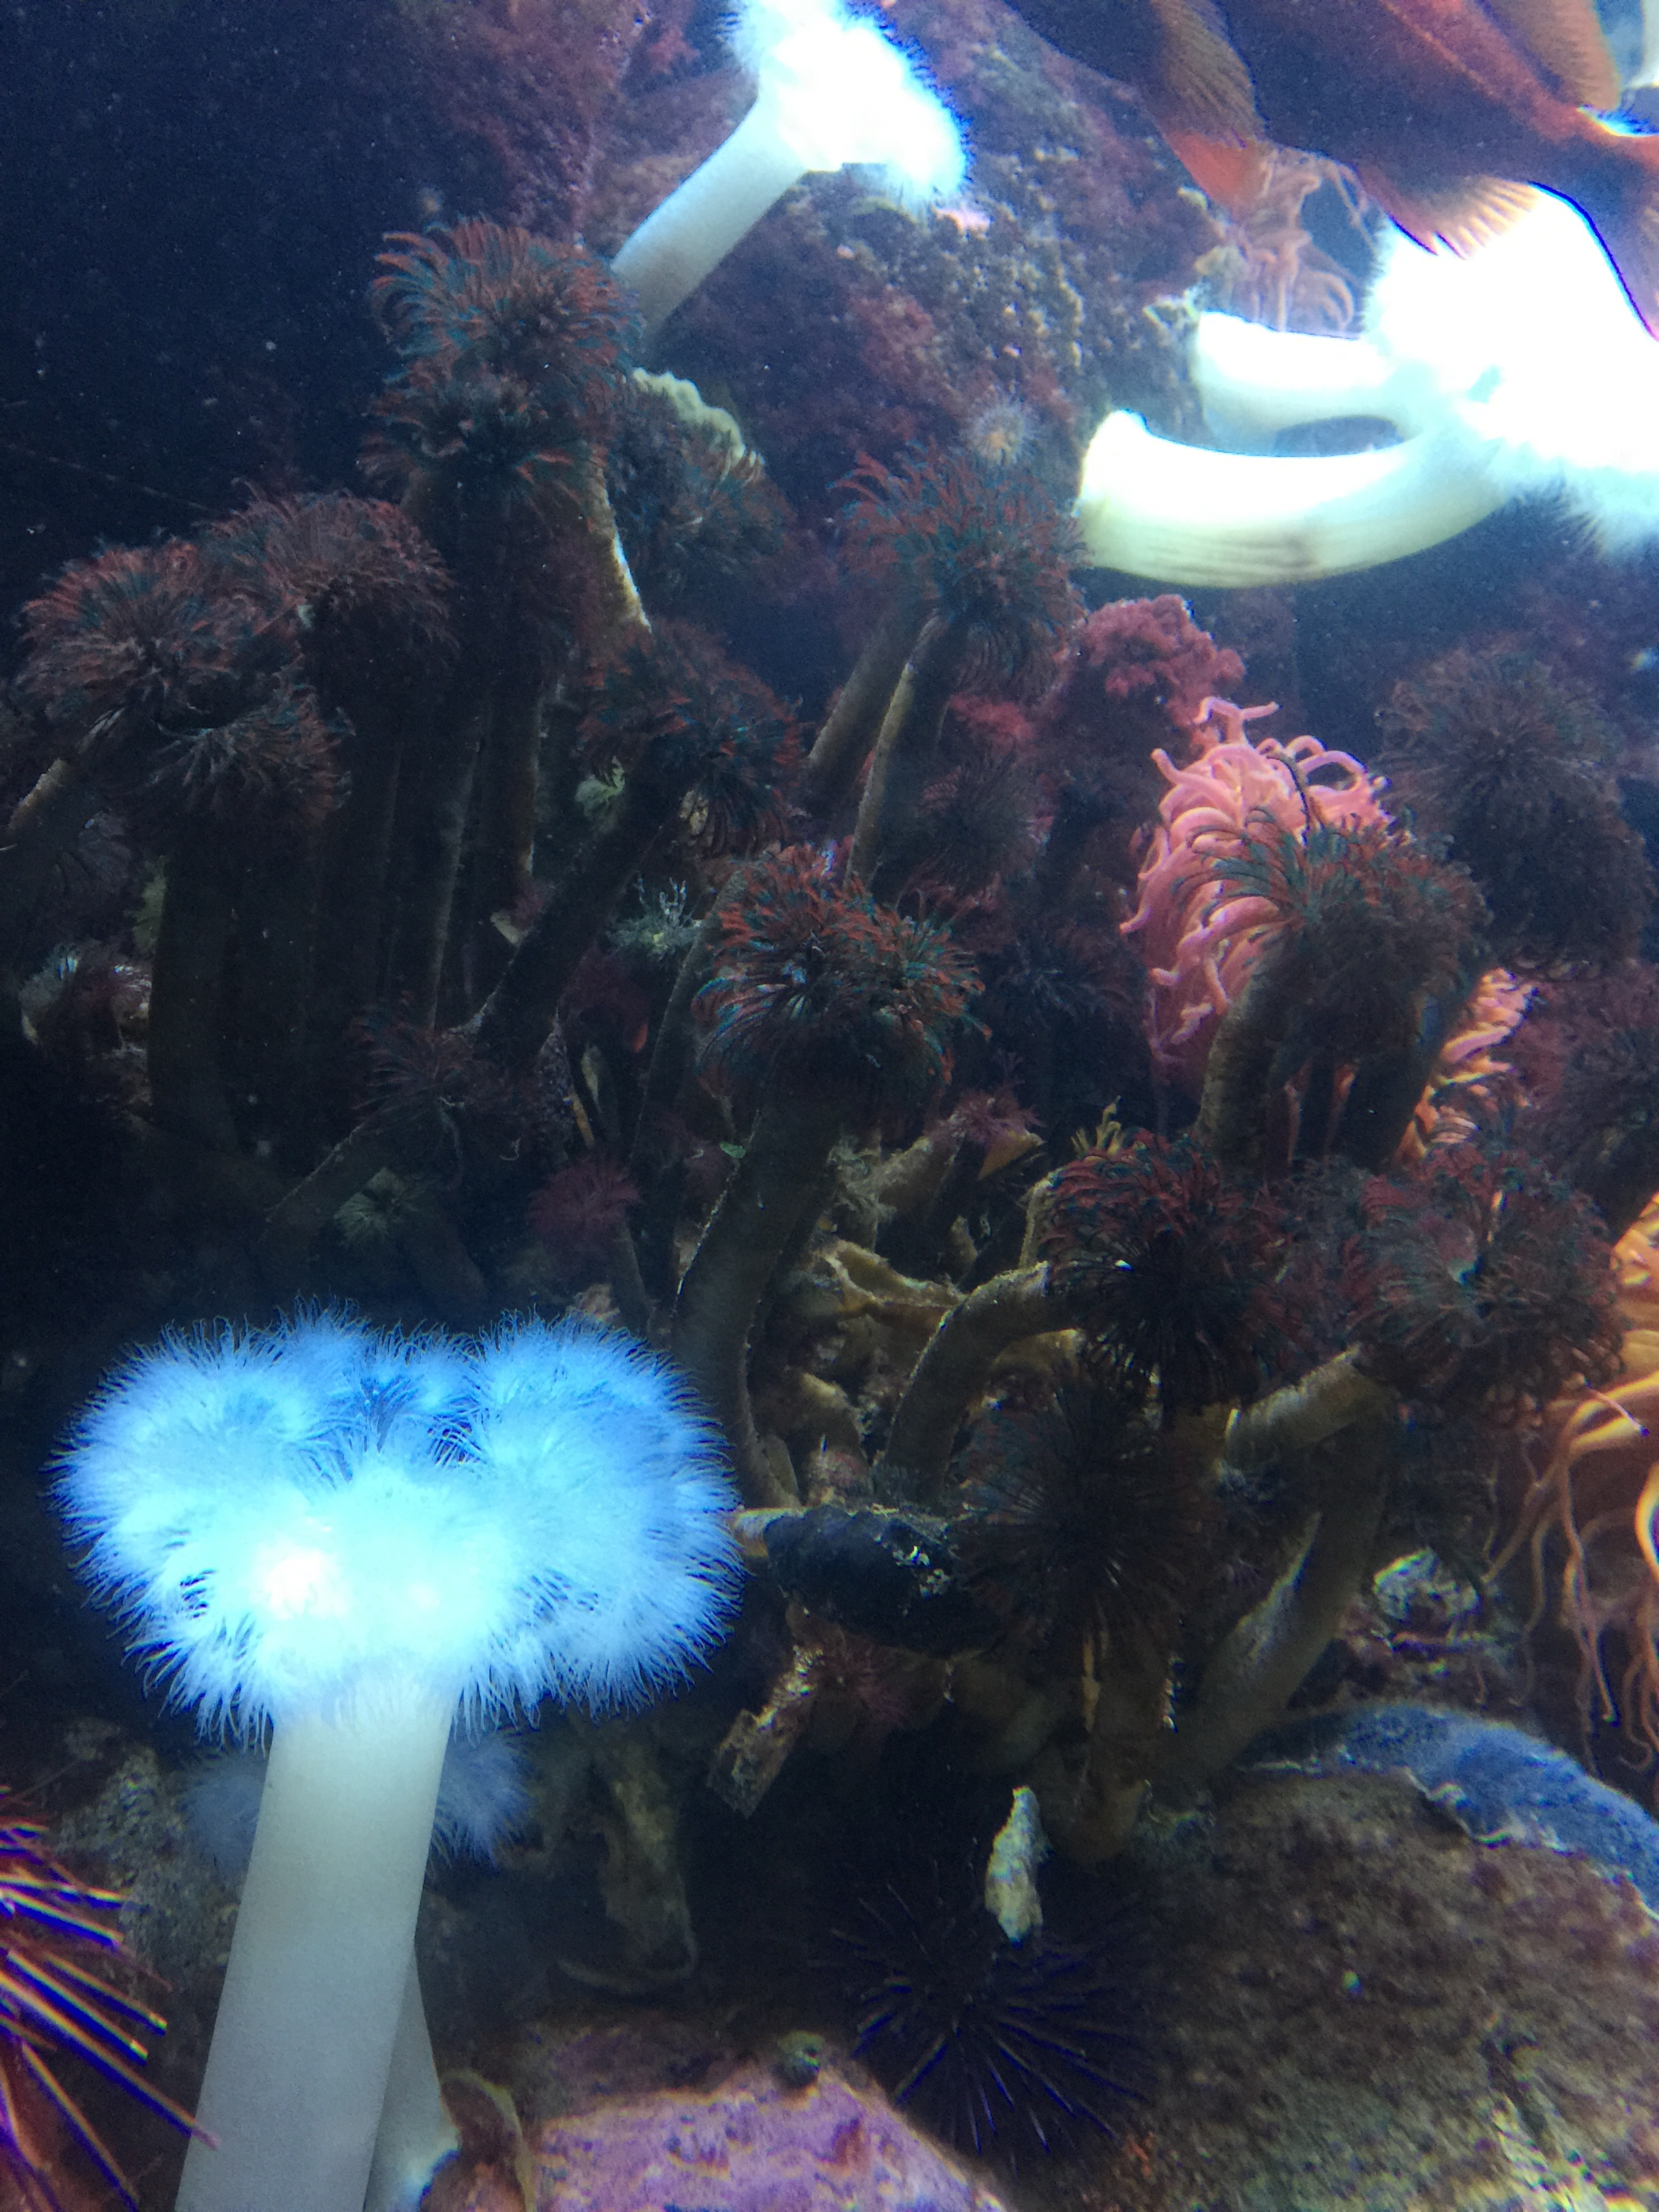
\includegraphics[width=0.7\linewidth]{./figures/porifera/metridium_live}

}

\caption{\emph{Metridium}.}\label{fig:metridum}
\end{figure}

\section{\texorpdfstring{View Prepared Slides of
\emph{Metridium}}{View Prepared Slides of Metridium}}\label{view-prepared-slides-of-metridium}

\begin{enumerate}
\def\labelenumi{\arabic{enumi}.}
\tightlist
\item
  \emph{Metridium} x.s. (Figure \ref{fig:metridiumxs})

  \begin{itemize}
  \tightlist
  \item
    Identify: tentacles, mouth, type of symmetry.
  \end{itemize}
\end{enumerate}

\begin{figure}

{\centering \includegraphics[width=0.7\linewidth]{./figures/porifera/metridium}

}

\caption{\emph{Metridium}.}\label{fig:metridiumxs}
\end{figure}

\section{View Living Organisms}\label{view-living-organisms-2}

\begin{enumerate}
\def\labelenumi{\arabic{enumi}.}
\tightlist
\item
  \emph{Hydra}
\end{enumerate}

\section{\texorpdfstring{\emph{Ctenophora}}{Ctenophora}}\label{ctenophora}

\href{https://en.wikipedia.org/wiki/Ctenophora}{Ctenophora} (singular
ctenophore; from the Greek kteis `comb' and pherō `carry'; commonly
known as comb jellies) is a phylum of invertebrate animals that live in
marine waters worldwide. They are notable for the groups of cilia they
use for swimming (commonly referred to as ``combs''), and they are the
largest animals that swim by means of cilia. Depending on the species,
adult ctenophores range from a few millimeters to 1.5 m in size. Only
100--150 species have been validated, and possibly another 25 have not
been fully described and named. The textbook examples are cydippids with
egg-shaped bodies and a pair of retractable tentacles fringed with
tentilla (``little tentacles'') that are covered with colloblasts,
sticky cells that capture prey.

The phylum has a wide range of body forms, including the flattened,
deep-sea platyctenids, in which the adults of most species lack combs,
and the coastal beroids, which lack tentacles and prey on other
ctenophores by using huge mouths armed with groups of large, stiffened
cilia that act as teeth. Almost all ctenophores are predators, taking
prey ranging from microscopic larvae and rotifers to the adults of small
crustaceans; the exceptions are juveniles of two species, which live as
parasites on the salps on which adults of their species feed. Most
species are hermaphrodites, and juveniles of at least some species are
capable of reproduction before reaching the adult size and shape. This
combination of hermaphroditism and early reproduction enables small
populations to grow at an explosive rate.

Early writers combined ctenophores with cnidarians into a single phylum
called Coelenterata on account of morphological similarities between the
two groups. Like cnidarians, the bodies of ctenophores consist of a mass
of jelly, with one layer of cells on the outside and another lining the
internal cavity. In ctenophores, however, these layers are two cells
deep, while those in cnidarians are only a single cell deep. Ctenophores
also resemble cnidarians in relying on water flow through the body
cavity for both digestion and respiration, as well as in having a
decentralized nerve net rather than a brain. However, genomic studies
have suggested that the neurons of Ctenophora, which differ in many ways
from other animal neurons, evolved independently from those of the other
animals, and increasing awareness of the differences between the groups
has persuaded more recent authors to classify the two as separate phyla.
The position of the ctenophores in the evolutionary family tree of
animals has long been debated, and the majority view at present, based
on molecular phylogenetics, is that cnidarians and bilaterians are more
closely related to each other than either is to ctenophores.

The traditional classification divides ctenophores into two classes,
those with tentacles (Tentaculata) and those without (Nuda). The Nuda
contains only one order (Beroida) and family (Beroidae), and two genera,
\emph{Beroe} (several species) and \emph{Neis} (one species).

The \emph{Tentaculata} are divided into the following eight orders:

\begin{enumerate}
\def\labelenumi{\arabic{enumi}.}
\tightlist
\item
  Cydippida, egg-shaped animals with long tentacles
\item
  Lobata, with paired thick lobes
\item
  Platyctenida, flattened animals that live on or near the
  sea-bed; most lack combs as adults, and use their pharynges as suckers
  to attach themselves to surfaces
\item
  Ganeshida, with a pair of small lobes round the mouth, but an
  extended pharynx like that of platyctenids
\item
  Cambojiida
\item
  Cryptolobiferida
\item
  Thalassocalycida, with short tentacles and a jellyfish-like
  ``umbrella''
\item
  Cestida, ribbon-shaped and the largest ctenophores
\end{enumerate}

Despite their soft, gelatinous bodies, fossils thought to represent
ctenophores, apparently with no tentacles but many more comb-rows than
modern forms, have been found as far back as the early Cambrian, about
515 million years ago.

Adults of most species can regenerate tissues that are damaged or
removed, although only platyctenids reproduce by cloning, splitting off
from the edges of their flat bodies fragments that develop into new
individuals.

Almost all species are hermaphrodites. Some are simultaneous
hermaphrodites, which can produce both eggs and sperm at the same time,
while others are sequential hermaphrodites, in which the eggs and sperm
mature at different times. The gonads are located in the parts of the
internal canal network under the comb rows, and eggs and sperm are
released via pores in the epidermis. Fertilization is generally
external, but some use internal fertilization and keep the eggs in brood
chambers until they hatch. Self-fertilization has occasionally been seen
in some species and it is thought that most of the hermaphroditic
species are self-fertile.

Development of the fertilized eggs is direct, in other words there is no
distinctive larval form. Juveniles of all groups are generally
planktonic, and in most species, resemble miniature adult cydippids,
gradually developing their adult body forms as they grow.

\section{Review Questions}\label{review-questions-3}

\begin{enumerate}
\def\labelenumi{\arabic{enumi}.}
\tightlist
\item
  What are animals?
\item
  What are porifera?
\item
  What are choanocytes?
\item
  What are cnidaria?
\item
  What are cnidocytes?
\item
  What is a statocyst?
\item
  What are ctenophora?
\item
  Ctenophora move by means of \underline{\phantom{answer}}.
\end{enumerate}
